\titlespacing*{\part}{0pt}{-20pt}{30pt} % to fix table and plot together on the first page (SEE RESTORE AT BOTTOM)
\titlespacing*{\chapter}{0pt}{-10pt}{30pt}

\part{Supervised Learning} % DIFF: top-level "part" is Supervised Learning (while "Linear Regression" is a chapter)
\label{part:supervised_learning}

\marginnote{From CS229 Fall 2020, Tengyu Ma, Andrew Ng, Moses Charikar, \& Christopher R\'e, Stanford University.}


Let's start by talking about a few examples of supervised learning problems.
Suppose we have a dataset giving the living areas and prices of 47 houses
from Portland, Oregon:

\begin{table}[!h]
  \centering
  \caption{
    \label{tab:houses} Housing prices in Portland, OR.
  }
  \begin{tabular}{cc}
    \toprule
    Living area (feet$^2$) & Price (1000\$s) \\
    \midrule
    2104 & 400 \\
    1600 & 330 \\
    2400 & 369 \\
    1416 & 232 \\
    3000 & 540 \\
    $\vdots$ & $\vdots$ \\
    \bottomrule
  \end{tabular}
\end{table}

\phantom{} % extra newline space

We can plot this data:
\begin{figure}
    \caption{
        \label{fig:houses} Housing prices in Portland, OR.
    }
    \begin{jlcode}
    p = let
        data = CSV.read("..\\data\\portland-houses.csv", DataFrame; header=["area", "bedrooms", "price"])
        X = data[:area]
        Y = data[:price] ./ 1000

        Axis(Plots.Scatter(X, Y, style="mark=x"), title="housing prices", xlabel="square feet", ylabel="price (in \\\$1000)", xmax=5000, ymax=800)
    end
    plot(p)
    \end{jlcode}
    \begin{center}
        \plot{fig/portland_houses}
    \end{center}
\end{figure}


Given data like this, how can we learn to predict the prices of other houses
in Portland, as a function of the size of their living areas?

To establish notation for future use, we'll use $x^{(i)}$ to denote the ``input''
variables (living area in this example), also called input \textbf{features}, and $y^{(i)}$
to denote the ``output'' or \textbf{target} variable that we are trying to predict
(price). A pair $(x^{(i)}, y^{(i)})$ is called a \textbf{training example}, and the dataset
that we'll be using to learn---a list of $n$ training examples $\{(x^{(i)}, y^{(i)} );\; i =
1,\ldots,n\}$---is called a \textbf{training set}. Note that the superscript ``$(i)$'' in the
notation is simply an index into the training set, and has nothing to do with
exponentiation. We will also use $\cal X$ denote the space of input values, and $\cal Y$
the space of output values. In this example, $\cal X = \cal Y = \bb R$.

To describe the supervised learning problem slightly more formally, our
goal is, given a training set, to learn a function $h: \cal X \mapsto \cal Y$ so that $h(x)$ is a
``good'' predictor for the corresponding value of $y$. For historical reasons, this
function $h$ is called a \textbf{hypothesis}. Seen pictorially, the process is therefore
like this:

\begin{figure}
\begin{center}
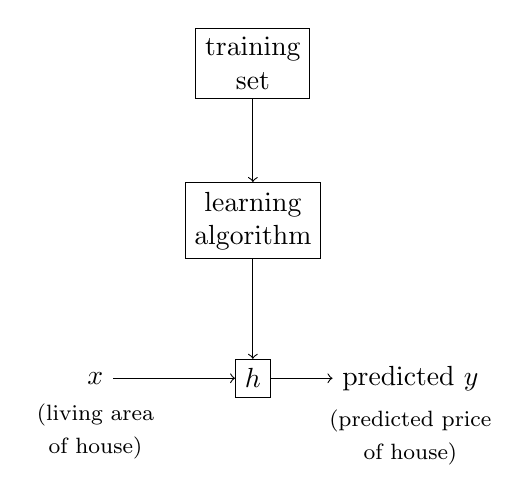
\begin{tikzpicture}[node distance=2cm, auto]
    \node [rectangle, align=center, draw] (training) {training\\set};
    \node [rectangle, align=center, draw, below of=training] (learning) {learning\\algorithm};
    \node [rectangle, align=center, draw, below of=learning] (h) {$h$};
    \node [left of=h, label={[align=center]below:\footnotesize (living area\\\footnotesize of house)}] (x) {$x$};
    \node [right of=h, label={[align=center]below:\footnotesize (predicted price\\\footnotesize of house)}] (y) {predicted $y$};

    \path [->, draw] (training) -- (learning);
    \path [->, draw] (learning) -- (h);
    \path [->, draw] (x) -- (h);
    \path [->, draw] (h) -- (y);
\end{tikzpicture}
\caption{\label{fig:hypothesis} Hypothesis diagram.}
\end{center}
\end{figure}

% TODO: get Francis Galton citation.
When the target variable that we're trying to predict is continuous, such
as in our housing example, we call the learning problem a \textbf{regression}\footnote{The term \textit{regression} was originally coined due to ``regressing'' to the mean (Francis Galton, 1886).} problem. % DIFF: regression term explanation.
When $y$ can take on only a small number of discrete values (such as
if, given the living area, we wanted to predict if a dwelling is a house or an
apartment, say), we call it a \textbf{classification} problem.


\chapter{Linear Regression}
\label{cha:linear_regression}

To make our housing example more interesting, let's consider a slightly richer
dataset in which we also know the number of bedrooms in each house:


\begin{table}[!h]
  \centering
  \caption{
    \label{tab:bedrooms} Housing prices with bedrooms in Portland, OR.
  }
  \begin{tabular}{ccc}
    \toprule
    Living area (feet$^2$) & \texttt{\#} Bedrooms & Price (1000\$s) \\
    \midrule
    2104 & 3 & 400 \\
    1600 & 3 & 330 \\
    2400 & 3 & 369 \\
    1416 & 2 & 232 \\
    3000 & 4 & 540 \\
    $\vdots$ & $\vdots$ & $\vdots$ \\
    \bottomrule
  \end{tabular}
\end{table}

Here, the $x$'s are two-dimensional vectors in $\bb R^2$. For instance, $x^{(i)}_1$
is the living area of the $i$-th house in the training set, and $x^{(i)}_2$
is its number of bedrooms.\footnote{In general, when designing a learning problem, it will be up to % DIFF: turned this parenthetical into a footnote
you to decide what features to choose, so if you are out in Portland gathering
housing data, you might also decide to include other features such as whether
each house has a fireplace, the number of bathrooms, and so on. We'll say
more about feature selection later, but for now let's take the features as
given.}

To perform supervised learning, we must decide how we're going to represent
functions/hypotheses $h$ in a computer. As an initial choice, let's say
we decide to approximate $y$ as a linear function of $x$:

\begin{equation}
    h_\theta(x) = \theta_0 + \theta_1 x_1 + \theta_2 x_2
\end{equation}

Here, the $\theta_i$'s are the \textbf{parameters} (also called \textbf{weights}) parameterizing the
space of linear functions mapping from $\cal X$ to $\cal Y$. When there is no risk of
confusion, we will drop the $\theta$ subscript in $h_\theta(x)$, and write it more simply as
$h(x)$. To simplify our notation, we also introduce the convention of letting
$x_0 = 1$ (this is the intercept term), so that
\begin{equation}
    h(x) = \sum_{i=0}^d \theta_i x_i = \theta^\top x\text{,} % DIFF: \top instead of ^T
\end{equation}
where on the right-hand side above we are viewing $\theta$ and $x$ both as vectors,
and here $d$ is the number of input variables (not counting $x_0$).

Now, given a training set, how do we pick, or learn, the parameters $\theta$?
One reasonable method seems to be to make $h(x)$ close to $y$, at least for
the training examples we have. To formalize this, we will define a function
that measures, for each value of the $\theta$'s, how close the $h(x^{(i)})$'s are to the
corresponding $y^{(i)}$'s. We define the \textbf{cost function}:

\begin{equation}
    J(\theta) = \frac 1 2 \sum_{i=1}^n \left( h_\theta(x^{(i)}) - y^{(i)} \right)^2\text{.}
\end{equation}

If you've seen linear regression before, you may recognize this as the familiar
least-squares cost function that gives rise to the \textbf{ordinary least squares}
regression model. Whether or not you have seen it previously, let's keep
going, and we'll eventually show this to be a special case of a much broader
family of algorithms.


\section{Least mean squares (LMS) algorithm} % DIFF: spelled out LMS

We want to choose $\theta$ so as to minimize $J(\theta)$. To do so, let's use a search
algorithm that starts with some ``initial guess'' for $\theta$, and that repeatedly
changes $\theta$ to make $J(\theta)$ smaller, until hopefully we converge to a value of
$\theta$ that minimizes $J(\theta)$. Specifically, let's consider the \textbf{gradient descent}
algorithm, which starts with some initial $\theta$, and repeatedly performs the
update:\footnote{This update is simultaneously performed for all values of $j = 0,\ldots,d$.} % DIFF: made parenthetical a footnote
%
\begin{equation}
    \theta_j \leftarrow \theta_j - \alpha \frac{\partial}{\partial \theta_j} J(\theta) % DIFF: Changed := to \leftarrow for update
\end{equation}
%
Here, $\alpha$ is called the \textbf{learning rate}. This is a very natural algorithm that
repeatedly takes a step in the direction of steepest decrease of $J$.

In order to implement this algorithm, we have to work out what is the
partial derivative term on the right hand side. Let's first work it out for the
case of if we have only one training example $(x,y)$, so that we can neglect
the sum in the definition of $J$. We have:

\begin{align*}
    \frac{\partial}{\partial \theta_j} J(\theta) &= \frac{\partial}{\partial \theta_j} \frac 1 2 \left( h_\theta(x) - y \right)^2\\
    &= 2 \cdot \frac 1 2 (h_\theta(x) - y) \cdot \frac{\partial}{\partial \theta_j} (h_\theta(x) - y) \\
    &= (h_\theta(x) - y) \cdot \frac{\partial}{\partial \theta_j} \left( \sum_{i=0}^d \theta_i x_i - y \right) \\
    &= (h_\theta(x) - y) x_j
\end{align*}

For a single training example, this gives the update rule:\footnote{We use the notation ``$a \leftarrow b$'' to denote an operation (in a computer program) in
which we set the value of a variable $a$ to be equal to the value of $b$ (something $:=$ is used). In other words, this
operation overwrites $a$ with the value of $b$. In contrast, we will write ``$a = b$'' when we are
asserting a statement of fact, that the value of $a$ is equal to the value of $b$.}

\begin{equation}
    \theta_j \leftarrow \theta_j + \alpha \left( y^{(i)} - h_\theta(x^{(i)}) \right) x^{(i)}_j \text{.} % DIFF: \leftarrow (:=)
\end{equation}

The rule is called the \textbf{LMS} update rule (LMS stands for ``least mean squares''),
and is also known as the \textbf{Widrow-Hoff} learning rule. This rule has several
properties that seem natural and intuitive. For instance, the magnitude of
the update is proportional to the \textbf{error} term $(y^{(i)} - h_\theta(x^{(i)}))$; thus, for
instance, if we are encountering a training example on which our prediction
nearly matches the actual value of $y^{(i)}$, then we find that there is little need
to change the parameters; in contrast, a larger change to the parameters will
be made if our prediction $h_\theta(x^{(i)})$ has a large error (i.e., if it is very far from
$y^{(i)}$).

We've derived the LMS rule for when there was only a single training % DIFF: we'd to we've
example. There are two ways to modify this method for a training set of
more than one example. The first is replace it with the following algorithm:

% DIFF: cleaned up this algorithm block (broke out the for loop).
\begin{algorithm}[ht]
    \caption{Gradient descent.}
    \label{alg:gd}
    \begin{algorithmic}
    \Repeat
        \For{every $j$}
            \State $\theta_j \leftarrow \theta_j + \alpha \displaystyle\sum\limits_{i=1}^n \left( y^{(i)} - h_\theta(x^{(i)}) \right) x^{(i)}_j$ %, \quad (for every $j$)
        \EndFor
    \Until{convergence}
    \end{algorithmic}
\end{algorithm}

By grouping the updates of the coordinates into an update of the vector
$\theta$, we can rewrite update \cref{alg:gd} in a slightly more succinct way:

\begin{algorithm}[ht]
    \caption{Gradient descent vectorized.}
    \label{alg:gd_vector}
    \begin{algorithmic}
    \Repeat
        \State $\theta \leftarrow \theta + \alpha \displaystyle\sum\limits_{i=1}^n \left( y^{(i)} - h_\theta(x^{(i)}) \right) x^{(i)}$
    \Until{convergence}
    \end{algorithmic}
\end{algorithm}

The reader can easily verify that the quantity in the summation in the
update rule above is just $\partial J(\theta) / \partial \theta_j$ (for the original definition of $J$).
So, this is simply gradient descent on the original cost function $J$. This method looks
at every example in the entire training set on every step, and is called \textbf{batch gradient descent}.
Note that, while gradient descent can be susceptible
to local minima in general, the optimization problem we have posed here
for linear regression has only one global, and no other local, optima; thus
gradient descent always converges (assuming the learning rate $\alpha$ is not too
large) to the global minimum. Indeed, $J$ is a convex quadratic function.


% TODO: Julia code (gradient descent—see alg4ai and "gradient_descent.jl")


\begin{example}
    \caption{\label{ex:gd} Gradient descent on a quadratic function.}

    Here is an example of gradient descent as it is run to minimize a quadratic
    function.

    \begin{jlcode}
    p = let
        @vars x, y
        f = x^2/2 + y^2
        plot_gradient_descent(f, initial=[48, 30], path_length=40)
    end
    plot(p)
    \end{jlcode}
    \begin{center}
        \plot{fig/gradient_descent}
    \end{center}

    The ellipses shown above are the contours of a quadratic function. Also
    shown is the trajectory taken by gradient descent, which was initialized at
    (48,30). The arrows in the figure (joined by straight lines) mark the successive % DIFF: changed $x$'s to arrows.
    values of $\theta$ that gradient descent went through.
\end{example}


\begin{example}
    % TODO: Generate \theta's directly from `linear_regression' (see plots-notebook.jl)
    When we run batch gradient descent to fit $\theta$ on our previous dataset,
    to learn to predict housing price as a function of living area. We obtain: % DIFF: split into two sentences.
    \begin{align*} % DIFF: put these in their own newlined equation block AND added \tag annotations.
        \theta_0 &= 71.27 \tag{intercept}\\
        \theta_1 &= 0.1345 \tag{slope}
    \end{align*}
    If we plot $h_\theta (x)$ as a function of $x$ (area), along
    with the training data, we obtain the following figure:

    \caption{
        % TODO I actually use linear regression here and not batch gradient descent.
        \label{ex:linear_regression} Best fit line using batch gradient descent on Portland, Oregon housing prices.
    }
    \begin{jlcode}
    p = let
        data = CSV.read("..\\data\\portland-houses.csv", DataFrame; header=["area", "bedrooms", "price"])
        X = data[:area]
        Y = data[:price] ./ 1000

        h = linear_regression(X, Y)

        p_data = Plots.Scatter(X, Y, style="mark=x")
        xn = (minimum(X) - 500):5000 # (maximum(X) + 500)

        p_fit = Plots.Linear(xn, h.(xn), style="blue, no marks")

        Axis([p_data, p_fit], title="housing prices", xlabel="square feet", ylabel="price (in \\\$1000)", xmin=first(xn), xmax=last(xn), ymax=800)
    end
    plot(p)
    \end{jlcode}
    \begin{center}
        \plot{fig/linear_regression}
    \end{center}

    % TODO: Generate \theta's directly from `linear_regression'
    If the number of bedrooms were included as one of the input features as well,
    we get $\theta_0 = 89.60, \theta_1 = 0.1392, \theta_2 = -8.738$.
\end{example}


% TODO: obtain these results with batch gradient descent.
The results in \cref{ex:linear_regression} were obtained with batch gradient descent. There is
an alternative to batch gradient descent that also works very well. Consider
the following algorithm:

% DIFF: Cleaned up the algorithm.
\begin{algorithm}[ht]
    \caption{Stochastic gradient descent.}
    \label{alg:sgd}
    \begin{algorithmic}
    \Repeat
        \For{$i = 1$ to $n$}
            \For{every $j$}
                \State $\theta_j \leftarrow \theta_j + \alpha \displaystyle\sum\limits_{i=1}^n \left( y^{(i)} - h_\theta(x^{(i)}) \right) x^{(i)}_j$ %, \quad (for every $j$)
            \EndFor
        \EndFor
    \Until{convergence}
    \end{algorithmic}
\end{algorithm}

By grouping the updates of the coordinates into an update of the vector
$\theta$, we can rewrite update in \cref{alg:sgd} in a slightly more succinct way:

\begin{equation}
    \theta \leftarrow \theta + \alpha \left( y^{(i)} - h_\theta^{(i)} \right) x^{(i)}
\end{equation}

In this algorithm, we repeatedly run through the training set, and each
time we encounter a training example, we update the parameters according
to the gradient of the error with respect to that single training example only.
This algorithm is called \textbf{stochastic gradient descent} (also \textbf{incremental
gradient descent}). Whereas batch gradient descent has to scan through
the entire training set before taking a single step---a costly operation if $n$ is
large---stochastic gradient descent can start making progress right away, and
continues to make progress with each example it looks at. Often, stochastic
gradient descent gets $\theta$ ``close'' to the minimum much faster than batch gradient
descent.\footnote{Note, however, that it may never ``converge'' to the minimum,
and the parameters $\theta$ will keep oscillating around the minimum of $J(\theta)$; but
in practice most of the values near the minimum will be reasonably good
approximations to the true minimum. By slowly letting the learning rate $\alpha$ decrease to
zero as the algorithm runs, it is also possible to ensure that the parameters will converge to
the global minimum rather than merely oscillate around the minimum.} % DIFF: combined parenthetical and footnote.
For these reasons, particularly when the training set is large,
stochastic gradient descent is often preferred over batch gradient descent.


\section{The normal equations}
\label{sec:the_normal_equations}

Gradient descent gives one way of minimizing $J$. Let's discuss a second way
of doing so, this time performing the minimization explicitly and without
resorting to an iterative algorithm. In this method, we will minimize $J$ by
explicitly taking its derivatives with respect to the $\theta_j$'s, and setting them to
zero. To enable us to do this without having to write reams of algebra and
pages full of matrices of derivatives, let's introduce some notation for doing
calculus with matrices.

\subsection{Matrix derivatives}
For a function $f : \bb R^{n \times d} \mapsto \bb R$ mapping from $n$-by-$d$ matrices to the real
numbers, we define the derivative of $f$ with respect to $A$ to be:

\begin{equation}
    \nabla_A f(A) = \begin{bmatrix}
        \frac{\partial f}{\partial A_{11}} & \cdots & \frac{\partial f}{\partial A_{1d}} \\
        \vdots & \ddots & \vdots \\
        \frac{\partial f}{\partial A_{n1}} & \cdots & \frac{\partial f}{\partial A_{nd}} \\
    \end{bmatrix}
\end{equation}

Thus, the gradient $\nabla_A f(A)$ is itself an $n$-by-$d$ matrix, whose $(i,j)$-element is
$\partial f / \partial A_{ij}$.

\begin{example}
    \caption{\label{ex:matrix_derivative}Matrix derivative.}

    For example, suppose $A =
    \begin{bmatrix}
        A_{11} & A_{12} \\
        A_{21} & A_{22}
    \end{bmatrix}$
    is a 2-by-2 matrix, and the function $f : \bb R^{2\times2} \mapsto \bb R$ is given by
    \begin{equation*}
        f(A) = \frac 3 2 A_{11} + 5 A_{12}^2 + A_{21}A_{22}\text{.}
    \end{equation*}
    Here, $A_{ij}$ denotes the $(i,j)$ entry of the matrix $A$. We then have:
    \begin{equation*}
        \nabla_A f(A) =
        \begin{bmatrix}
            \frac 3 2 & 10 A_{12} \\
            A_{22} & A_{21}
        \end{bmatrix}
    \end{equation*}
\end{example}


\subsection{Least squares revisited}

% TODO: \vec \theta ???? (CHANGE THROUGHOUT)

Armed with the tools of matrix derivatives, let us now proceed to find in
closed-form the value of $\theta$ that minimizes $J(\theta)$. We begin by re-writing $J$ in
matrix-vector notation. % DIFF: changed from "matrix-vectorial" to "matrix-vector"

% DIFF: bold-faced matrix $\mat X$
Given a training set, define the \textbf{design matrix} $\mat X$ to be the $n$-by-$d$ matrix
(actually $n$-by-$(d + 1)$, if we include the intercept term) that contains the % DIFF: added (...) around d+1
training examples' input values in its rows:

% DIFF: \top not ^T, bold-faced matrix (from here on out.)
\begin{equation}
    \mat X = \begin{bmatrix}
        \text{--- } (x^{(1)})^\top \text{ ---} \\
        \text{--- } (x^{(2)})^\top \text{ ---} \\
        \vdots \\
        \text{--- } (x^{(n)})^\top \text{ ---}
    \end{bmatrix}
\end{equation}
% DIFF: bold-face vector notation (not above-arrow, from here on out.)
Also, let $\vec y$ be the $n$-dimensional vector containing all the target values from
the training set:
\begin{equation}
    \vec y = \begin{bmatrix}
        y^{(1)} \\
        y^{(2)} \\
        \vdots \\
        y^{(n)}
    \end{bmatrix}
\end{equation}
Now, since $h_\theta(x^{(i)}) = (x^{(i)})^\top \theta$, we can easily verify that
\begin{align*}
    \mat X \theta - \vec y &= \begin{bmatrix}
        (x^{(1)})^\top \theta \\
        \vdots \\
        (x^{(n)})^\top \theta
    \end{bmatrix}
    -
    \begin{bmatrix}
        y^{(1)} \\    
        \vdots \\
        y^{(n)}    
    \end{bmatrix}\\
    &= \begin{bmatrix}
        h_\theta(x^{(1)}) - y^{(1)} \\
        \vdots \\
        h_\theta(x^{(n)}) - y^{(n)}
    \end{bmatrix}\text{.}
\end{align*}
Thus, using the fact that for a vector $z$, we have that $z^\top z = \sum_i z_i^2$:
\begin{align*}
    \frac 1 2 (\mat X \theta - \vec y)^\top (\mat X \theta - \vec y) &= \frac 1 2 \sum_{i=1}^n \left( h_\theta(x^{(i)}) - y^{(i)} \right)^2 \\
    &= J(\theta)
\end{align*}
Finally, to minimize $J$, let's find its derivative with respect to $\theta$. Hence:
\begin{align*}
    \nabla_\theta J(\theta) &= \nabla_\theta \frac 1 2 (\mat X \theta - \vec y)^\top (\mat X \theta - \vec y) \\
                            &= \frac 1 2 \nabla_\theta \left( (\mat X \theta)^\top \mat X \theta - (\mat X \theta)^\top \vec y - \vec y^\top (\mat X \theta) + \vec y^\top \vec y \right) \\
                            &= \frac 1 2 \nabla_\theta \left( \theta^\top (\mat X^\top \mat X) \theta - \vec y^\top (\mat X \theta) - \vec y^\top (\mat X \theta) \right) \tag{$a^\top b = b^\top a$} \\
                            &= \frac 1 2 \nabla_\theta \left( \theta^\top (\mat X^\top \mat X) \theta - 2 (\mat X^\top \vec y)^\top \theta \right) \\
                            &= \frac 1 2 \left( 2\mat X^\top \mat X \theta - 2 \mat X^\top \vec y \right) \tag{$\nabla_x b^\top x = b$ and $\nabla_x x^\top A x = 2 A x$ for sym. $A$} \\
                            &= \mat X^\top \mat X \theta - \mat X^\top \vec y
\end{align*}
% DIFF: Moved "third step" and "fifth step" explanations to \tags
To minimize $J$, we set its derivatives to zero, and obtain the \textbf{normal equations}:
\begin{equation}
    \mat X^\top \mat X \theta = \mat X^\top \vec y
\end{equation}
Thus, the value of $\theta$ that minimizes $J(\theta)$ is given in closed form by the equation:
\footnote{Note that in the this step, we are implicitly assuming that $\mat X^\top \mat X$ is an invertible
matrix. This can be checked before calculating the inverse. If either the number of
linearly independent examples is fewer than the number of features, or if the features
are not linearly independent, then $\mat X^\top \mat X$ will not be invertible. Even in such cases, it is
possible to ``fix'' the situation with additional techniques, which we skip here for the sake of simplicty.}
\begin{equation}
    \theta = (\mat X^\top \mat X)^{-1} \mat X^\top \vec y
\end{equation}


\section{Probabilistic interpretation}
When faced with a regression problem, why might linear regression, and
specifically why might the least-squares cost function $J$, be a reasonable
choice? In this section, we will give a set of probabilistic assumptions, under
which least-squares regression is derived as a very natural algorithm.

Let us assume that the target variables and the inputs are related via the
equation
\begin{equation}
    y^{(i)} = \theta^\top x^{(i)} + \epsilon^{(i)}\text{,}
\end{equation}
where $\epsilon^{(i)}$ is an error term that captures either unmodeled effects (such as
if there are some features very pertinent to predicting housing price, but
that we'd left out of the regression), or random noise. Let us further assume
that the $\epsilon^{(i)}$ are distributed IID (independently and identically distributed)
according to a Gaussian distribution (also called a Normal distribution) with
mean zero and some variance $\sigma^2$. We can write this assumption as % DIFF: removed quotes
$\epsilon^{(i)} \sim \cal N(0, \sigma^2)$, i.e. the density of $\epsilon^{(i)}$ is given by
\begin{equation}
    p(\epsilon^{(i)}) = \frac{1}{\sqrt{2\pi}\sigma} \exp \left( - \frac{(\epsilon^{(i)})^2}{2\sigma^2} \right)\text{.}
\end{equation}
This implies that
\begin{equation}
    p(y^{(i)} \mid x^{(i)}; \theta) = \frac{1}{\sqrt{2\pi}\sigma} \exp \left( - \frac{(y^{(i)} - \theta^\top x^{(i)})^2}{2\sigma^2} \right)\text{.}
\end{equation}
The notation ``$p(y^{(i)} \mid x^{(i)}; \theta)$'' indicates that this is the distribution of $y^{(i)}$
given $x^{(i)}$ and parameterized by $\theta$. Note that we should not condition on $\theta$
(i.e. ``$p(y^{(i)} \mid x^{(i)}, \theta)$''), since $\theta$ is not a random variable. We can also write the
distribution of $y^{(i)}$ as $(y^{(i)} \mid x^{(i)}; \theta) \sim \cal N(\theta^\top x^{(i)}, \sigma^2)$. % DIFF: added parens

Given $\mat X$ (the design matrix, which contains all the $x^{(i)}$'s) and $\theta$, what
is the distribution of the $y^{(i)}$'s? The probability of the data is given by
$p(\vec y \mid \mat X; \theta)$. This quantity is typically viewed a function of $\vec y$ (and perhaps $\mat X$),
for a fixed value of $\theta$. When we wish to explicitly view this as a function of
$\theta$, we will instead call it the \textbf{likelihood} function:
\begin{equation}
    L(\theta) = L(\theta; \mat X, \vec y) = p(\vec y \mid \mat X; \theta) %DIFF: removed period.
\end{equation}
Note that by the independence assumption on the $\epsilon^{(i)}$'s (and hence also the
$y^{(i)}$'s given the $x^{(i)}$'s), this can also be written as %DIFF: added "as"
\begin{align}
    L(\theta) &= \prod_{i=1}^n p(y^{(i)} \mid x^{(i)}; \theta)\\
              &= \prod_{i=1}^n \frac{1}{\sqrt{2\pi}\sigma} \exp \left( - \frac{(y^{(i)} - \theta^\top x^{(i)})^2}{2\sigma^2} \right)\text{.}
\end{align}
Now, given this probabilistic model relating the $y^{(i)}$'s and the $x^{(i)}$'s, what
is a reasonable way of choosing our best guess of the parameters $\theta$? The
principal of \textbf{maximum likelihood} says that we should choose $\theta$ so as to
make the data as high probability as possible---i.e. we should choose $\theta$ to
maximize $L(\theta)$.

Instead of maximizing $L(\theta)$, we can also maximize any strictly increasing
function of $L(\theta)$. In particular, the derivations will be a bit simpler if we
instead maximize the \textbf{log likelihood} $\ell(\theta)$:
\begin{align*}
    \ell(\theta) &= \log L(\theta) \\
    &= \log \prod_{i=1}^n \frac{1}{\sqrt{2\pi}\sigma} \exp \left( - \frac{(y^{(i)} - \theta^\top x^{(i)})^2}{2\sigma^2} \right) \\
    &= \sum_{i=1}^n \log \frac{1}{\sqrt{2\pi}\sigma} \exp \left( - \frac{(y^{(i)} - \theta^\top x^{(i)})^2}{2\sigma^2} \right) \\
    &= n \log \frac{1}{\sqrt{2\pi}\sigma} - \frac{1}{\sigma^2} \cdot \frac{1}{2} \sum_{i=1}^n \left(y^{(i)} - \theta^\top x^{(i)} \right)^2 %DIFF: no period.
\end{align*}
Hence, maximizing $\ell(\theta)$ gives the same answer as minimizing
\begin{equation*}
    \frac 1 2 \sum_{i=1}^n \left( y^{(i)} - \theta^\top x^{(i)} \right)^2\text{,}
\end{equation*}
which we recognize to be $J(\theta)$, our original least-squares cost function.

\paragraph{To summarize} Under the previous probabilistic assumptions on the data,
least-squares regression corresponds to finding the maximum likelihood estimate
of $\theta$. This is thus one set of assumptions under which least-squares regression
can be justified as a very natural method that's just doing maximum
likelihood estimation.\footnote{Note however that the probabilistic assumptions are
by no means necessary for least-squares to be a perfectly good and rational
procedure, and there may---and indeed there are---other natural assumptions
that can also be used to justify it.} % DIFF: footnote instead of parenthetical

Note also that, in our previous discussion, our final choice of $\theta$ did not
depend on what was $\sigma^2$, and indeed we'd have arrived at the same result
even if $\sigma^2$ were unknown. We will use this fact again later, when we talk
about the exponential family and generalized linear models.


\section{Locally weighted linear regression}
Consider the problem of predicting $y$ from $x \in \bb R$. The leftmost figure below
shows the result of fitting a $y = \theta_0 + \theta_1 x$ to a dataset. We see that the data
doesn't really lie on straight line, and so the fit is not very good.

\begin{figure*}
    \caption{
        \label{fig:polynomoial_regression} Polynomial regression with different $k$-order fits.
    }
    \begin{jlcode}
    p = let
        D = [(1,1), (2,2), (3,3), (4,3.25), (5,3.5), (6,3.75)]

        g = GroupPlot(3, 1, style="width=0.3\\textwidth")
        push!(g, plot_polynomial_regression(D, 1))
        push!(g, plot_polynomial_regression(D, 2))
        push!(g, plot_polynomial_regression(D, 5))
        g
    end
    plot(p)
    \end{jlcode}
    \begin{center}
        \plot{fig/polynomial_regression}
    \end{center}
\end{figure*}

Instead, if we had added an extra feature $x^2$, and fit $y = \theta_0 + \theta_1 x + \theta_2 x^2$,
then we obtain a slightly better fit to the data. (See middle figure) Naively, it
might seem that the more features we add, the better. However, there is also
a danger in adding too many features: The rightmost figure is the result of
fitting a 5-th order polynomial $y = \sum_{j=0}^5 \theta_j x^j$. We see that even though the
fitted curve passes through the data perfectly, we would not expect this to
be a very good predictor of, say, housing prices ($y$) for different living areas
($x$). Without formally defining what these terms mean, we'll say the figure
on the left shows an instance of \textbf{underfitting}---in which the data clearly
shows structure not captured by the model---and the figure on the right is
an example of \textbf{overfitting}.\footnote{Later in this class, when we talk about learning
theory we'll formalize some of these notions, and also define more carefully
just what it means for a hypothesis to be good or bad.} % DIFF: footnote from parenthetical

As discussed previously, and as shown in \cref{fig:polynomoial_regression}, the choice of %DIFF: \cref
features is important to ensuring good performance of a learning algorithm.
(When we talk about model selection, we'll also see algorithms for automatically
choosing a good set of features.) In this section, let us briefly talk
about the \textbf{locally weighted linear regression} (LWR) algorithm which, assuming
there is sufficient training data, makes the choice of features less critical.
This treatment will be brief, since you'll get a chance to explore some of the
properties of the LWR algorithm yourself in the homework.

In the original linear regression algorithm, to make a prediction at a query
point $x$ (i.e. to evaluate $h(x)$), we would: % DIFF: removed comma in i.e.
\begin{enumerate}
    \item Fit $\theta$ to minimize $\sum_i \left( y^{(i)} - \theta^\top x^{(i)} \right)^2$.
    \item Output $\theta^\top x$.
\end{enumerate}

In contrast, the locally weighted linear regression algorithm does the following:
\begin{enumerate}
    \item Fit $\theta$ to minimize $\sum_i w^{(i)} \left(y^{(i)} - \theta^\top x^{(i)} \right)^2$.
    \item Output $\theta^\top x$.
\end{enumerate}

Here, the $w^{(i)}$'s are non-negative valued \textbf{weights}. Intuitively, if $w^{(i)}$ is large
for a particular value of $i$, then in picking $\theta$ we'll try hard to make $(y^{(i)} - \theta^\top x^{(i)})^2$ small.
If $w^{(i)}$ is small, then the $(y^{(i)} - \theta^\top x^{(i)})^2$ error term will be
pretty much ignored in the fit.

A fairly standard choice for the weights is:% DIFF: footnote has equation blocks (moved w^{(i)} into sentence, outside of equations)
\footnote{If $x$ is vector-valued, the weights $w^{(i)}$ can be generalized to
\[\exp \left( - \frac{(x^{(i)} - x)^\top (x^{(i)} - x)}{2\tau^2} \right)\]
or
\[\exp \left( - \frac{(x^{(i)} - x)^\top \Sigma^{-1} (x^{(i)} - x)}{2\tau^2} \right)\]
for appropriate choices of $\tau$ or $\Sigma$.}
\begin{equation}
    w^{(i)} = \exp \left( - \frac{(x^{(i)} - x)^2}{2\tau^2} \right)
\end{equation}
Note that the weights depend on the particular point $x$ at which we're trying
to evaluate $x$. Moreover, if $\lvert x^{(i)} - x \rvert$ is small, then $w^{(i)}$ is close to 1; and
if $\lvert x^{(i)} - x \rvert$ is large, then $w^{(i)}$ is small. Hence, $\theta$ is chosen giving a much
higher ``weight'' to the (errors on) training examples close to the query point
$x$.\footnote{Note also that while the formula for the weights takes a form that is
cosmetically similar to the density of a Gaussian distribution, the $w^{(i)}$'s do
not directly have anything to do with Gaussians, and in particular the $w^{(i)}$
are not random variables, normally distributed or otherwise.} % DIFF: footnote instead of parenthetical
The parameter $\tau$ controls how quickly the weight of a training example falls off with distance
of its $x^{(i)}$ from the query point $x$; $\tau$ is called the \textbf{bandwidth} parameter, and
is also something that you'll get to experiment with in your homework.

Locally weighted linear regression is the first example we're seeing of a
\textbf{non-parametric} algorithm. The (unweighted) linear regression algorithm
that we saw earlier is known as a \textbf{parametric} learning algorithm, because
it has a fixed, finite number of parameters (the $\theta_i$'s), which are fit to the
data. Once we've fit the $\theta_i$'s and stored them away, we no longer need to
keep the training data around to make future predictions. In contrast, to
make predictions using locally weighted linear regression, we need to keep
the entire training set around. The term ``non-parametric'' (roughly) refers
to the fact that the amount of stuff we need to keep in order to represent the
hypothesis $h$ grows linearly with the size of the training set.



\chapter{Classification and Logistic Regression}
\label{cha:classification_logistic_regression}

Let's now talk about the classification problem. This is just like the regression
problem, except that the values $y$ we now want to predict take on only
a small number of discrete values. For now, we will focus on the \textbf{binary
classification} problem in which $y$ can take on only two values, $0$ and $1$.
(Most of what we say here will also generalize to the multiple-class case.)
For instance, if we are trying to build a spam classifier for email, then $x^{(i)}$
may be some features of a piece of email, and $y$ may be $1$ if it is a piece
of spam mail, and $0$ otherwise. The class $0$ is also called the \textbf{negative class}, and $1$ % DIFF: added "The class" to the sentence (don't start with numbers...)
the \textbf{positive class}, and they are sometimes also denoted by the symbols ``$-$''
and ``$+$''. Given $x^{(i)}$, the corresponding $y^{(i)}$ is also called the \textbf{label} for the
training example.

\section{Logistic regression} % NOTE Section 5.

\titlespacing*{\part}{0pt}{50pt}{40pt} % RESTORE
\titlespacing*{\chapter}{0pt}{50pt}{40pt} % RESTORE

We could approach the classification problem ignoring the fact that $y$ is
discrete-valued, and use our old linear regression algorithm to try to predict
$y$ given $x$. However, it is easy to construct examples where this method
performs very poorly. Intuitively, it also doesn't make sense for $h_\theta (x)$ to take
values larger than 1 or smaller than 0 when we know that $y \in \{0,1\}$.

To fix this, let's change the form for our hypotheses $h_\theta (x)$. We will choose
\[
h_\theta (x) = g(\theta^\top x) = \frac{1}{1 + e^{-\theta^\top x}}
\]
where
\[
g(z) = \frac{1}{1 + e^{-z}}
\]
is called the \textbf{logistic function} or the \textbf{sigmoid function}. Here is a plot
showing $g(z)$:

\begin{figure}
    \caption{
        \label{fig:sigmoid} Sigmoid function (i.e. logistic).
    }
    \begin{jlcode}
    p = let
        σ(z) = 1/(1 + exp(-z))
        X = -5:0.1:5
        Plots.Linear(X, σ.(X), style="blue, no marks")
    end
    plot(p)
    \end{jlcode}
    \begin{center}
        \plot{fig/sigmoid}
    \end{center}
\end{figure}

Notice that $g(z)$ tends towards $1$ as $z \to \infty$, and $g(z)$ tends towards $0$ as
$z \to -\infty$. Moreover, $g(z)$, and hence also $h(x)$, is always bounded between
$0$ and $1$. As before, we are keeping the convention of letting $x_0 = 1$, so that $\theta^\top x = \theta_0 + \sum_{j=1}^{d} \theta_j x_j$.

For now, let's take the choice of $g$ as given. Other functions that smoothly
increase from 0 to 1 can also be used, but for a couple of reasons that we'll see
later (when we talk about GLMs, and when we talk about generative learning
algorithms), the choice of the logistic function is a fairly natural one. Before
moving on, here's a useful property of the derivative of the sigmoid function,
which we write as $g'$:
\begin{align}
    g'(z) &= \frac{d}{dz}\frac{1}{1 + e^{-z}}\\
    &= \frac{1}{(1 + e^{-z})^2} (e^{-z})\\
    &= \frac{1}{(1 + e^{-z})} \cdot \left( 1 - \frac{1}{(1 + e^{-z})} \right)\\
    &= g(z)(1 - g(z))
\end{align}

So, given the logistic regression model, how do we fit $\theta$ for it? Following
how we saw least squares regression could be derived as the maximum likelihood
estimator under a set of assumptions, let's endow our classification
model with a set of probabilistic assumptions, and then fit the parameters
via maximum likelihood.

Let us assume that
\begin{align*}
    P(y = 1 \mid x;\theta) &= h_\theta (x)\\
    P(y = 0 \mid x;\theta) &= 1 - h_\theta (x)
\end{align*}
Note that this can be written more compactly as
\begin{equation}
    p(y \mid x;\theta) = (h_\theta (x))^y (1 - h_\theta (x))^{1-y}
\end{equation}
Assuming that the $n$ training examples were generated independently, we
can then write down the likelihood of the parameters as
\begin{align}
    L(\theta) &= p(\vec y \mid X;\theta)\\
    &= \prod^n_{i=1} p(y^{(i)} \mid x^{(i)} ;\theta)\\
    &= \prod^n_{i=1} \left( h_\theta(x^{(i)}) \right)^{y^{(i)}} \left( 1 - h_\theta (x^{(i)}) \right)^{1-y^{(i)}}
\end{align}
As before, it will be easier to maximize the log likelihood:
\begin{align}
    \ell(\theta) &= \log L(\theta)\\
    &= \sum_{i=1}^n y^{(i)} \log h(x^{(i)}) + (1 - y^{(i)})\log(1 - h(x^{(i)}))
\end{align}

How do we maximize the likelihood? Similar to our derivation in the case
of linear regression, we can use gradient ascent. Written in vectorial notation,
our updates will therefore be given by $\theta := \theta + \alpha \nabla_\theta \ell(\theta)$. (Note the positive
rather than negative sign in the update formula, since we're maximizing,
rather than minimizing, a function now.) Let's start by working with just
one training example $(x,y)$, and take derivatives to derive the stochastic
gradient ascent rule:
\begin{align}
    \frac{\partial}{\partial \theta_j}\ell(\theta) &=
    \left(y \frac{1}{g(\theta^\top x)} - (1-y) \frac{1}{1-g(\theta^\top x)} \right) \frac{\partial}{\partial \theta_j}g(\theta^\top x)\\
    &= \left(y \frac{1}{g(\theta^\top x)} - (1-y) \frac{1}{1-g(\theta^\top x)} \right) g(\theta^\top x) (1 - g(\theta^\top x)) \frac{\partial}{\partial \theta_j}\theta^\top x\\
    &= \left(y (1 - g(\theta^\top x)) - (1-y) g(\theta^\top x)\right) x_j\\
    &= (y - h_\theta(x)) x_j
\end{align}
Above, we used the fact that $g'(z) = g(z)(1 - g(z))$. This therefore gives us
the stochastic gradient ascent rule
\begin{equation}
    \theta_j := \theta_j + \alpha \left( y^{(i)} - h_\theta (x^{(i)}) \right) x^{(i)}_j
\end{equation}
If we compare this to the LMS update rule, we see that it looks identical; but
this is not the same algorithm, because $h_\theta (x^{(i)})$ is now defined as a non-linear
function of $\theta^\top x^{(i)}$. Nonetheless, it's a little surprising that we end up with
the same update rule for a rather different algorithm and learning problem.
Is this coincidence, or is there a deeper reason behind this? We'll answer this
when we get to GLM models.


\section{Digression: The perceptron learning algorithm} % TYPO: algorithn
We now digress to talk briefly about an algorithm that's of some historical
interest, and that we will also return to later when we talk about learning
theory. Consider modifying the logistic regression method to ``force'' it to
output values that are either 0 or 1 or exactly. To do so, it seems natural to
change the definition of g to be the threshold function:
\begin{equation}
    g(z) = \begin{cases}
        1 & \text{if } z \ge 0\\
        0 & \text{if } z < 0
    \end{cases}
\end{equation}
If we then let $h_\theta (x) = g(\theta^\top x)$ as before but using this modified definition of
$g$, and if we use the update rule
\begin{equation}
    \theta_j := \theta_j + \alpha \left( y^{(i)} - h_\theta (x^{(i)} ) \right) x^{(i)}_j    
\end{equation}
then we have the perceptron learning algorithm. % TYPO.

In the 1960s, this ``perceptron'' was argued to be a rough model for how
individual neurons in the brain work. Given how simple the algorithm is, it
will also provide a starting point for our analysis when we talk about learning
theory later in this class. Note however that even though the perceptron may
be cosmetically similar to the other algorithms we talked about, it is actually
a very different type of algorithm than logistic regression and least squares
linear regression; in particular, it is difficult to endow the perceptron's predic-
tions with meaningful probabilistic interpretations, or derive the perceptron
as a maximum likelihood estimation algorithm.


\section{Another algorithm for maximizing $\ell(\theta)$}

Returning to logistic regression with $g(z)$ being the sigmoid function, let's
now talk about a different algorithm for maximizing $\ell(\theta)$.

To get us started, let's consider Newton's method for finding a zero of a
function. Specifically, suppose we have some function $f : \mathbb R \mapsto \mathbb R$, and we
wish to find a value of $\theta$ so that $f(\theta) = 0$. Here, $\theta \in \mathbb R$ is a real number.
Newton's method performs the following update:
\begin{equation}
    \theta := \theta - \frac{f(\theta)}{f'(\theta)}
\end{equation}
This method has a natural interpretation in which we can think of it as
approximating the function $f$ via a linear function that is tangent to $f$ at
the current guess $\theta$, solving for where that linear function equals to zero, and
letting the next guess for $\theta$ be where that linear function is zero.

Here's a picture of the Newton's method in action:
\begin{figure*}
    \caption{
        \label{fig:newtons_method} Newton's method for two steps.
    }
    \begin{jlcode}
    p = plot_newtons_method()
    plot(p)
    \end{jlcode}
    \begin{center}
        \plot{fig/newtons_method}
    \end{center}
\end{figure*}

In the leftmost figure, we see the function f plotted along with the line
$y = 0$. We're trying to find $\theta$ so that $f(\theta) = 0$; the value of $\theta$ that achieves this
is about 1.3. Suppose we initialized the algorithm with $\theta = 4.5$. Newton's
method then fits a straight line tangent to $f$ at $\theta = 4.5$, and solves for the
where that line evaluates to 0. (Middle figure.) This give us the next guess
for $\theta$, which is about 2.8. The rightmost figure shows the result of running
one more iteration, which the updates $\theta$ to about 1.8. After a few more
iterations, we rapidly approach $\theta = 1.3$.

Newton's method gives a way of getting to $f(\theta) = 0$. What if we want to
use it to maximize some function $\ell$? The maxima of $\ell$ correspond to points
where its first derivative $\ell'(\theta)$ is zero. So, by letting $f(\theta) = \ell'(\theta)$, we can use
the same algorithm to maximize $\ell$, and we obtain update rule:
\begin{equation}
    \theta := \theta - \frac{\ell'(\theta)}{\ell^{\prime\prime}(\theta)}.
\end{equation}
(Something to think about: How would this change if we wanted to use
Newton's method to minimize rather than maximize a function?)

Lastly, in our logistic regression setting, $\theta$ is vector-valued, so we need to
generalize Newton's method to this setting. The generalization of Newton's
method to this multidimensional setting (also called the Newton-Raphson
method) is given by:
\begin{equation}
    \theta := \theta - H^{-1} \nabla_\theta \ell(\theta).
\end{equation}
Here, $\nabla_\theta \ell(\theta)$ is, as usual, the vector of partial derivatives of $\ell(\theta)$ with respect
to the $\theta_i$'s; and $H$ is an $d$-by-$d$ matrix (actually, $d+1$-by-$d+1$, assuming that
we include the intercept term) called the \textbf{Hessian}, whose entries are given by
\begin{equation}
    H ij = \frac{\partial^2 \ell(\theta)}{\partial\theta_i \partial\theta_j}.
\end{equation}

Newton's method typically enjoys faster convergence than (batch) gradient
descent, and requires many fewer iterations to get very close to the
minimum. One iteration of Newton's can, however, be more expensive than
one iteration of gradient descent, since it requires finding and inverting an
$d$-by-$d$ Hessian; but so long as $d$ is not too large, it is usually much faster
overall. When Newton's method is applied to maximize the logistic regression
log likelihood function $\ell(\theta)$, the resulting method is also called \textbf{Fisher
scoring}.



\chapter{Generalized Linear Models}

\marginnote{The presentation of the material in this section takes inspiration from Michael I.
Jordan, \textit{Learning in graphical models} (unpublished book draft), and also McCullagh and
Nelder, \textit{Generalized Linear Models} (2nd ed.).}

So far, we've seen a regression example, and a classification example. In the
regression example, we had $y \mid x; \theta \sim \mathcal{N}(\mu, \sigma^2)$, and in the classification one,
$y \mid x; \theta \sim \operatorname{Bernoulli}(\phi)$, for some appropriate definitions of $\mu$ and $\phi$ as functions
of $x$ and $\theta$. In this section, we will show that both of these methods are
special cases of a broader family of models, called \textit{Generalized Linear Models}
(GLMs). We will also show how other models in the GLM family can be
derived and applied to other classification and regression problems.

\section{The exponential family}
To work our way up to GLMs, we will begin by defining exponential family
distributions. We say that a class of distributions is in the exponential family
if it can be written in the form:
\[
p(y; \eta) = b(y)\exp(\eta^\top T(y) - a(\eta)) \label{eq:glm}
\]
Here, $\eta$ is called the \textbf{natural parameter} (also called the \textbf{canonical parameter})
of the distribution; $T(y)$ is the \textbf{sufficient statistic} (for the distributions
we consider, it will often be the case that $T(y) = y$); and $a(\eta)$ is the \textbf{log
partition function}. The quantity $e^{-a(\eta)}$ essentially plays the role of a normalization
constant, that makes sure the distribution $p(y;\eta)$ sums/integrates
over $y$ to 1.
\marginnote{MLE w.r.t. $\eta$ is concave $\rightarrow$ (neg. log-likelihood is convex)}

A fixed choice of $T$, $a$ and $b$ defines a family (or set) of distributions that
is parameterized by $\eta$; as we vary $\eta$, we then get different distributions within
this family.

We now show that the Bernoulli and the Gaussian distributions are examples
of exponential family distributions. The Bernoulli distribution with
mean $\phi$, written $\operatorname{Bernoulli}(\phi)$, specifies a distribution over $y \in \{0,1\}$, so that
$p(y = 1;\phi) = \phi; p(y = 0;\phi) = 1 - \phi$. As we vary $\phi$, we obtain Bernoulli
distributions with different means. We now show that this class of Bernoulli
distributions, ones obtained by varying $\phi$, is in the exponential family; i.e.,
that there is a choice of $T$, $a$ and $b$ so that \ref{eq:glm} becomes exactly the
class of Bernoulli distributions.

We write the Bernoulli distribution as:
\begin{align}
    p(y;\phi) &= \phi^y (1 - \phi)^{1-y}\\
              &= \exp(y \log\phi + (1 - y)\log(1 - \phi))\\
              &= \exp\left( y\left( \log\left(\frac{\phi}{1-\phi}\right)\right) + \log(1-\phi)\right).
\end{align}
Thus, the natural parameter is given by $\eta = \log(\phi/(1 - \phi))$. Interestingly, if
we invert this definition for $\eta$ by solving for $\phi$ in terms of $\eta$, we obtain $\phi =
1/(1 + e^{-\eta})$. This is the familiar sigmoid function! This will come up again
when we derive logistic regression as a GLM. To complete the formulation
of the Bernoulli distribution as an exponential family distribution, we also
have:
\begin{align*}
    T(y) &= y\\
    a(\eta) &= -\log(1 - \phi)\\
            &= \log(1 + e^{\eta})\\
    b(y) &= 1    
\end{align*}
This shows that the Bernoulli distribution can be written in the form of
\ref{eq:glm}, using an appropriate choice of $T$, $a$ and $b$.

Let's now move on to consider the Gaussian distribution. Recall that,
when deriving linear regression, the value of $\sigma^2$ had no effect on our final
choice of $\theta$ and $h_\theta (x)$. Thus, we can choose an arbitrary value for $\sigma^2$ without
changing anything. To simplify the derivation below, let's set $\sigma^2 = 1$.\footnote{If we leave $\sigma^2$ as a variable, the Gaussian distribution can also be shown to be in the exponential family, where $\eta \in \mathbb R^2$ is now a 2-dimension vector that depends on both $\mu$ and
$\sigma$. For the purposes of GLMs, however, the $\sigma^2$ parameter can also be treated by considering
a more general definition of the exponential family: $p(y;\eta,\tau) = b(a,\tau)\exp((\eta^\top T(y) - a(\eta))/c(\tau))$.
Here, $\tau$ is called the \textbf{dispersion parameter}, and for the Gaussian, $c(\tau) = \sigma^2$;
but given our simplification above, we won't need the more general definition for the
examples we will consider here.}
We then have:
\begin{align}
    p(y;\mu) &= \frac{1}{\sqrt{2\pi}}\exp\left(-\frac{1}{2} (y - \mu)^2\right)\\
             &= \frac{1}{\sqrt{2\pi}}\exp\left(-\frac{1}{2} y^2 \right) \cdot  \exp\left(\mu y - \frac{1}{2}\mu^2\right)
\end{align}
Thus, we see that the Gaussian is in the exponential family, with
\begin{align*}
    \eta &= \mu\\
    T(y) &= y\\
    a(\eta) &= \mu^2 / 2\\
            &= \eta^2 / 2\\
    b(y) &= (1 / \sqrt{2\pi})\exp(-y^2 / 2).
\end{align*}
There're many other distributions that are members of the exponential family:
The multinomial (which we'll see later), the Poisson (for modelling
count-data; also see the problem set); the gamma and the exponential
(for modelling continuous, non-negative random variables, such as time-intervals);
the beta and the Dirichlet (for distributions over probabilities);
and many more. In the next section, we will describe a general ``recipe''
for constructing models in which $y$ (given $x$ and $\theta$) comes from any of these
distributions.


\section{Constructing GLMs}
\marginnote{Inference is easy:
\[
\mathbb E[y; \eta] = \frac{\partial}{\partial \eta} a(\eta)
\]
(log partition of exp. family).
}
Suppose you would like to build a model to estimate the number $y$ of customers
arriving in your store (or number of page-views on your website) in
any given hour, based on certain features $x$ such as store promotions, recent
advertising, weather, day-of-week, etc. We know that the Poisson distribution
usually gives a good model for numbers of visitors. Knowing this, how
can we come up with a model for our problem? Fortunately, the Poisson is an
exponential family distribution, so we can apply a Generalized Linear Model
(GLM). In this section, we will we will describe a method for constructing
GLM models for problems such as these.

More generally, consider a classification or regression problem where we
would like to predict the value of some random variable $y$ as a function of
$x$. To derive a GLM for this problem, we will make the following three
assumptions about the conditional distribution of $y$ given $x$ and about our
model:
\begin{enumerate}
    \item $y \mid x;\theta \sim \operatorname{ExponentialFamily}(\eta)$. I.e., given $x$ and $\theta$, the distribution of
$y$ follows some exponential family distribution, with parameter $\eta$.
    \item Given $x$, our goal is to predict the expected value of $T(y)$ given $x$.
    In most of our examples, we will have $T(y) = y$, so this means we
    would like the prediction $h(x)$ output by our learned hypothesis $h$ to
    satisfy $h(x) = \mathbb E[y \mid x]$. (Note that this assumption is satisfied in the
    choices for $h_\theta (x)$ for both logistic regression and linear regression. For
    instance, in logistic regression, we had $h_\theta (x) = p(y = 1 \mid x;\theta) = 0 \cdot p(y =
        0 \mid x;\theta) + 1 \cdot p(y = 1 \mid x;\theta) = \mathbb E[y \mid x;\theta]$.)

    \item The natural parameter $\eta$ and the inputs $x$ are related linearly: $\eta = \theta^\top x$.
    (Or, if $\eta$ is vector-valued, then $\eta_i = \theta^\top_i x$.)
\end{enumerate}

The third of these assumptions might seem the least well justified of
the above, and it might be better thought of as a ``design choice'' in our
recipe for designing GLMs, rather than as an assumption per se. These
three assumptions/design choices will allow us to derive a very elegant class
of learning algorithms, namely GLMs, that have many desirable properties
such as ease of learning. Furthermore, the resulting models are often very
effective for modelling different types of distributions over $y$; for example, we
will shortly show that both logistic regression and ordinary least squares can
both be derived as GLMs.

\subsection{Ordinary Least Squares}
To show that ordinary least squares is a special case of the GLM family
of models, consider the setting where the target variable $y$ (also called the
\textbf{response variable} in GLM terminology) is continuous, and we model the
conditional distribution of $y$ given $x$ as a Gaussian $\mathcal N(\mu,\sigma^2)$. (Here, $\mu$ may
depend $x$.) So, we let the $\operatorname{ExponentialFamily}(\eta)$ distribution above be
the Gaussian distribution. As we saw previously, in the formulation of the
Gaussian as an exponential family distribution, we had $\mu = \eta$. So, we have
\begin{align*}
    h_\theta (x) &= \mathbb E[y \mid x;\theta]\\
    &= \mu\\
    &= \eta\\
    &= \theta^\top x.
\end{align*}
The first equality follows from Assumption 2, above; the second equality
follows from the fact that $y \mid x;\theta \sim \mathcal N(\mu,\sigma^2)$, and so its expected value is given
by $\mu$; the third equality follows from Assumption 1 (and our earlier derivation
showing that $\mu = \eta$ in the formulation of the Gaussian as an exponential
family distribution); and the last equality follows from Assumption 3.

\subsection{Logistic Regression}
We now consider logistic regression. Here we are interested in binary classification,
so $y \in \{0,1\}$. Given that $y$ is binary-valued, it therefore seems natural
to choose the Bernoulli family of distributions to model the conditional distribution
of $y$ given $x$. In our formulation of the Bernoulli distribution as
an exponential family distribution, we had $\phi = 1/(1 + e^{-\eta})$. Furthermore,
note that if $y \mid x;\theta \sim \operatorname{Bernoulli}(\phi)$, then $\mathbb E[y \mid x;\theta] = \phi$. So, following a similar
derivation as the one for ordinary least squares, we get:
\begin{align*}
    h_\theta (x) &= \mathbb E[y \mid x;\theta]\\
    &= \phi\\
    &= 1/(1 + e^{-\eta})\\
    &= 1/(1 + e^{-\theta^\top x})    
\end{align*}
So, this gives us hypothesis functions of the form $h_\theta (x) = 1/(1 + e^{-\theta^\top x})$. If
you are previously wondering how we came up with the form of the logistic
function $1/(1 + e^{-z})$, this gives one answer: Once we assume that $y$ conditioned
on $x$ is Bernoulli, it arises as a consequence of the definition of GLMs
and exponential family distributions.

To introduce a little more terminology, the function $g$ giving the distribution's
mean as a function of the natural parameter ($g(\eta) = \mathbb E[T(y); \eta]$)
is called the \textbf{canonical response function}. Its inverse, $g^{-1}$, is called the
\textbf{canonical link function}. Thus, the canonical response function for the
Gaussian family is just the identity function; % TYPO? identity not "identify"?
and the canonical response function for the Bernoulli is the logistic function.\footnote{Many texts use $g$ to denote the link function, and $g^{-1}$
to denote the response function; but the notation we're using here, inherited from the early machine learning literature,
will be more consistent with the notation used in the rest of the class.}

\subsection{Softmax Regression}
Let's look at one more example of a GLM. Consider a classification problem
in which the response variable $y$ can take on any one of $k$ values, so $y \in
\{1,2,\ldots,k\}$. For example, rather than classifying email into the two classes
spam or not-spam---which would have been a binary classification problem---
we might want to classify it into three classes, such as spam, personal mail,
and work-related mail. The response variable is still discrete, but can now
take on more than two values. We will thus model it as distributed according
to a multinomial distribution.

Let's derive a GLM for modelling this type of multinomial data. To do
so, we will begin by expressing the multinomial as an exponential family
distribution.

To parameterize a multinomial over $k$ possible outcomes, one could use
$k$ parameters $\phi_1 ,\ldots,\phi_k$ specifying the probability of each of the outcomes.
However, these parameters would be redundant, or more formally, they would
not be independent (since knowing any $k-1$ of the $\phi_i$'s uniquely determines
the last one, as they must satisfy $\sum_{i=1}^k \phi_i = 1$). So, we will instead parameterize
the multinomial with only $k - 1$ parameters, $\phi_1,\ldots,\phi_{k-1}$, where
$\phi_i = p(y = i;\phi)$, and $p(y = k;\phi) = 1 - \sum_{i=1}^{k-1} \phi_i$. For notational convenience,
we will also let $\phi_k = 1 - \sum_{i=1}^{k-1} \phi_i$, but we should keep in mind that this is
not a parameter, and that it is fully specified by $\phi_1,\ldots,\phi_{k-1}$.

To express the multinomial as an exponential family distribution, we will
define $T(y) \in \mathbb R^{k-1}$ as follows:
\begin{equation*}
    T(1) = \begin{bmatrix}1\\0\\0\\\vdots\\0\end{bmatrix},
    T(2) = \begin{bmatrix}0\\1\\0\\\vdots\\0\end{bmatrix},
    \cdots,
    T(k-1) = \begin{bmatrix}0\\0\\0\\\vdots\\1\end{bmatrix},
    T(k) = \begin{bmatrix}0\\0\\0\\\vdots\\0\end{bmatrix},
\end{equation*}
Unlike our previous examples, here we do \textit{not} have $T(y) = y$; also, $T(y)$ is
now a $k - 1$ dimensional vector, rather than a real number. We will write
$(T(y))_i$ to denote the $i$-th element of the vector $T(y)$.
We introduce one more very useful piece of notation. An indicator function
$\mathbb{1}\{\cdot\}$ takes on a value of 1 if its argument is true, and 0 otherwise
($\mathbb{1}\{\texttt{True}\} = 1$, $\mathbb{1}\{\texttt{False}\} = 0$). For example, $\mathbb{1}\{2 = 3\} = 0$, and $\mathbb{1}\{3 =
5 - 2\} = 1$. So, we can also write the relationship between $T(y)$ and $y$ as
$(T(y))_i = \mathbb{1}\{y = i\}$. (Before you continue reading, please make sure you understand
why this is true!) Further, we have that $\mathbb E[(T(y))_i] = P(y = i) = \phi_i$.

We are now ready to show that the multinomial is a member of the
exponential family. We have:
\begin{align*}
    p(y; \phi) &= \phi_1^{\mathbb{1}\{y=1\}} \phi_2^{\mathbb{1}\{y=2\}} \cdots \phi_k^{\mathbb{1}\{y=k\}}\\
               &= \phi_1^{\mathbb{1}\{y=1\}} \phi_2^{\mathbb{1}\{y=2\}} \cdots \phi_k^{1 - \sum_{i=1}^{k-1}\mathbb{1}\{y=i\}}\\
               &= \phi_1^{(T(y))_1} \phi_2^{(T(y))_2} \cdots \phi_k^{1 - \sum_{i=1}^{k-1}(T(y))_i}\\
               &= \exp\left((T(y))_i \log(\phi_1) + (T(y))_2 \log(\phi_2) + \cdots + \left(1 - \sum_{i=1}^{k-1} (T(y))_i \right) \log(\phi_k) \right)\\
               &= \exp\left((T(y))_i \log(\phi_1/\phi_k) + (T(y))_2 \log(\phi_2/\phi_k) + \cdots + (T(k))_{k-1} \log(\phi_{k-1}/\phi_k) + \log(\phi_k)\right)\\
               &= b(y) \exp(\eta^\top T(y) - a(\eta))
\end{align*}
where
\begin{align*}
    \eta &= \begin{bmatrix} \log(\phi_1 / \phi_k) \\ \log(\phi_2 / \phi_k) \\ \vdots \\ \log(\phi_{k-1}/\phi_k) \end{bmatrix},\\
    a(\eta) &= - \log(\phi_k)\\
    b(y) &= 1.
\end{align*}
This completes our formulation of the multinomial as an exponential family
distribution.

The link function is given (for $i = 1,\ldots,k$) by:
\[
\eta_i = \log \frac{\phi_i}{\phi_k}
\]
For convenience, we have also defined $\eta_k = \log(\phi_k / \phi_k) = 0$. To invert the
link function and derive the response function, we therefore have that
\begin{align}
    e^{\eta_i} &= \frac{\phi_i}{\phi_k}\\
    \phi_k e^{\eta_i} &= \phi_i\label{eq:resp_fnc}\\
    \phi_k \sum_{i=1}^k e^{\eta_i} &= \sum_{i=1}^k \phi_i = 1
\end{align}
This implies that $\phi_k = 1 / \sum_{i=1}^k e^{\eta_i}$, which can be substituted back into \cref{eq:resp_fnc} to give the response function
\[
\phi_i = \frac{e^{\eta_i}}{\sum_{j=1}^k e^{\eta_j}}
\]
This function mapping from the $\eta$'s to the $\phi$'s is called the \textbf{softmax} function.

To complete our model, we use Assumption 3, given earlier, that the $\eta_i$'s
are linearly related to the $x$'s. So, have $\eta_i = \theta^\top_i x$ (for $i = 1,\ldots, k-1$),
where $\theta_1,\ldots, \theta_{k-1} \in \mathbb R^{d+1}$ are the parameters of our model. For notational
convenience, we can also define $\theta_k = 0$, so that $\eta_k = \theta^\top_k x = 0$, as given
previously. Hence, our model assumes that the conditional distribution of $y$
given $x$ is given by:
\begin{align}
    p(y=1 \mid x; \theta) &= \phi_i\\
                          &= \frac{e^{\eta_i}}{\sum_{j=1}^k e^{\eta_j}}\\
                          &= \frac{e^{\theta^\top_i x}}{\sum_{j=1}^k e^{\theta^\top_j x}} \label{eq:cond_distr}
\end{align}
This model, which applies to classification problems where $y \in \{1,...,k\}$, is
called \textbf{softmax regression}. It is a generalization of logistic regression.

Our hypothesis will output:
\begin{align}
    h_\theta(x) &= \mathbb E \left[ T(y) \mid x; \theta \right]\\
                &= \mathbb E \left[\begin{matrix}\mathbb{1}\{y=1\}\\\mathbb{1}\{y=2\}\\\vdots\\\mathbb{1}\{y=k-1\}\end{matrix} \mid x; \theta \right]\\    
                &= \begin{bmatrix}\phi_1\\\phi_2\\\vdots\\\phi_{k-1}\end{bmatrix}\\
                &= \begin{bmatrix}\frac{\exp(\theta^\top_1 x)}{\sum_{j=1}^k \exp(\theta^\top_j x)}\\\frac{\exp(\theta^\top_2 x)}{\sum_{j=1}^k \exp(\theta^\top_j x)}\\\vdots\\\frac{\exp(\theta^\top_{k-1} x)}{\sum_{j=1}^k \exp(\theta^\top_j x)}\end{bmatrix}
\end{align}
In other words, our hypothesis will output the estimated probability that
$p(y = i \mid x;\theta)$, for every value of $i = 1,\ldots,k$. (Even though $h_\theta (x)$ as defined
above is only $k - 1$ dimensional, clearly $p(y = k \mid x;\theta)$ can be obtained as $1 - \sum^{k-1}_{i=1} \phi_i$.)

Lastly, let's discuss parameter fitting. Similar to our original derivation
of ordinary least squares and logistic regression, if we have a training set of
$n$ examples $\{(x^{(i)} ,y^{(i)} );i = 1,\ldots,n\}$ and would like to learn the parameters
$\theta_i$ of this model, we would begin by writing down the log-likelihood
\begin{align}
    \ell(\theta) &= \sum_{i=1}^n \log p(y^{(i)} \mid x^{(i)}; \theta)\\
                 &= \sum_{i=1}^n \log \prod_{l=1}^k \left( \frac{e^{\theta^\top_l x^{(i)}}}{\sum_{j=1}^k e^{\theta^\top_j x^{(i)}}} \right) ^{\mathbb{1}\{y^{(i)} = l\}}
\end{align}
To obtain the second line above, we used the definition for $p(y \mid x;\theta)$ given
in \ref{eq:cond_distr}. We can now obtain the maximum likelihood estimate of
the parameters by maximizing $\ell(\theta)$ in terms of $\theta$, using a method such as
gradient ascent or Newton's method.